\begin{comment}
	\pagebreak
\end{comment}

\section{Normalizing Flows}
\begin{comment}
	\textbf{Goal:} What we want is a model that combines the tractable likelihoods from AR models with the latent space of VAE.\\
\end{comment}

\textbf{Variable change 1D:} $p_x(x) = p_z(h(x)) \abs{h(x)}$\\
\textbf{2D:} $\int \int f(x,y) dxdy = \int \int f(g(u,v), h(u,v)) J(u,v) dudv$\\
\begin{comment}
	The probabilitstic mass must be preserved!\\
\end{comment}

\textbf{Normalizing Flow:} $f: \R \rightarrow \R$, cont. and invertible\\
$p_X(x; \theta) = p_Z(f_\theta^{-1}(x)) \abs{det(\frac{\partial f_\theta^{-1}(x)}{\partial x})}
= p_z(f^{-1}(x)) \abs{det(\frac{\partial f(z)}{\partial z})}^{-1}$\\
\begin{comment}
	\textbf{Example Linear transformation:} $z = Ax \\
	\Rightarrow p_x(x) = p_z(A^{-1}x) \abs{det(A^{-1})}$\\
	\Note{Not every NN works to model f:}\\
	\begin{itemize}
	\item must be differentiable
	\item must be invertible
	\item must preserve dimensionality
	\item jacobian must be computed efficiently	
	\end{itemize}
	
	\begin{Figure}
 		\centering
 		
\includegraphics[width=\linewidth]{graphic/normflow-mapping}
 		\captionof{figure}{Normalizing Flow mapping}
	\end{Figure}
\end{comment}

\textbf{Coupling:} $(y_A; y_B)^T = (h(x^A, \beta(x^B)); x^B)^T$  $|$ h:elemnt, $\beta$:NN\\
$(x^A; x^B)^T = (h^{-1}(y^A; \beta(y^B)); y^B)^T$, $J = ((h'; h'f'),(0;1))$\\
\begin{comment}
	\Note{The Jacobian is triangular.} This allows computation of det in $\BigO(d)$, instead of $\BigO(d^3)$\\
	\Note{$\beta$ does not have to be invertible}\\
	
	\begin{Figure}
 		\centering
 		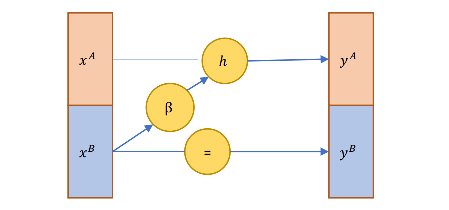
\includegraphics[width=\linewidth]{graphic/normflow-coupling}
 		\captionof{figure}{Normalizing Flow coupling layer}
	\end{Figure}
\end{comment}

\textbf{Composition:} $p_X(x; \theta) = p_Z(f_\theta^{-1}(x)) \prod_k \abs{det(\frac{\partial f_\theta^{-1}(x)}{\partial x})}$\\
\begin{comment}
	For $x = f(z) = f_k \circ f_{k-1} \circ \circ \circ f_2 \circ f_1(z)$\\
\end{comment}

\textbf{Train:}$log p_x(D) = \sum_{x}^{D} (log p_z(f^{-1}(x)) +  \sum_k \log \abs{det(\frac{\partial f^{-1}(x)}{\partial x})})$\\
\textbf{Inference:} draw $z \sim p_z(.)$, $\whx = f(z)$\\
\begin{comment}
	The whole point of this is that we want to draw $z \sim \cN(0,I)$ and then learn the transformation to create really complex x\\
	-\\ 
	-\\
\end{comment}

\textbf{Model:} $x_i \rightarrow squeeze \rightarrow n.flow \rightarrow split \rightarrow z_i (\text{repeat } L-1)\\
\rightarrow squeeze \rightarrow n.flow \rightarrow z_L$\\
\begin{comment}
	The flow step is repeated K times and consists of 
	\begin{itemize}
	\item actnorm (like batch normalization)
	\item 1x1 conv
	\item affine coupling layer	
	\end{itemize}

\end{comment}
